El objetivo de este capítulo es demostrar las partes importantes o de interés de la implementación y como se ha logrado la realización de lo mencionado en capítulos anteriores.

\section{El monorepo del proyecto}

Una de las cosas fundamentales a la hora de crear este proyecto era conseguir dividir el proyecto en varias secciones sin dificultar el trabajar con ellas a la vez. Es por esto que se decidió usar un monorepo para guardar el proyecto y aprovechar de ciertas herramientas para facilitar su uso. Como herramienta principal para gestionar el monorepo se decidió usar \verb|turborepo| \cite{turborepo}, debido a que es uno de las más populares y de los que más rendimiento tienen a la hora de construir las aplicaciones. Además de usar turborepo, se decidió aprovechar una de las opciones que trae el gestor de paquetes \verb|pnpm| \cite{pnpm}, los \verb|worspaces| \cite{pnpm-workspaces}, la cual permite unir varios proyectos dentro del mismo repositorio y compartir las dependencias entre ellos. Por último, se utilizó la herramienta \verb|changesets| \cite{changesets} para el control de versiones de los diferentes paquetes y proyectos del monorepo.

\section{El inicializador de {\tt adastra}}

Como se dijo anteriormente en el apartado de diseño se ha creado un paquete llamado \verb|create-adastra-lms|, que sirve como punto de inicio para crear un proyecto con AdAstra. La función principal de este paquete se muestra en la figura \ref{fig:adastraCreateMain}. Lo primero que se realiza es la extracción de los argumentos pasados al programa, para luego crear un objeto \verb|context|, que proporciona los datos que necesitará la aplicación, en función de estos argumentos. En caso de que se haya pasado como argumento una \textit{flag} de ayuda, como \verb|-h| o \verb|--help|, se mostrará el menú de ayuda como resultado, se puede ver en la figura \ref{fig:adastraCreateHelp}. Para finalizar, se ejecutarán los diferentes pasos de la ejecución, encapsulados dentro de un array, que en este caso se tratan de diferentes funciones asíncronas que se llamarán una después de otra. Para facilitar el proceso de creación de este paquete se ha usado, una librería del framework de \verb|Astro| \cite{astro} llamada \verb|@astrojs/cli-kit| \cite{astro-cli} que suministra de diferentes utilidades que sirven para facilitar la creación de un programa de cli, como la petición de un prompt o las personalización de los mensajes. 

\begin{figure}
    \begin{lstlisting}[language=Javascript]
        export const main = async () => {
          const clearArgv = process.argv.slice(2).filter((arg) => arg !== "--");
          const context = getContext(clearArgv);
          if (context.help) return help();
        
          const steps = [projectName, template, dependecies, git, next];
        
          for (const step of steps) {
            await step(context);
          }
        
          exit();
        };
    \end{lstlisting}
    \caption{Función principal de create-adastra-lms}
    \label{fig:adastraCreateMain}
\end{figure}

\begin{figure}
    \centering
    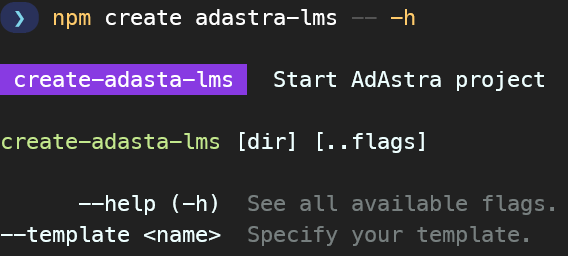
\includegraphics{images/adastraHelp.png}
    \caption{Salida del flag de ayuda de create-adastra-lms}
    \label{fig:adastraCreateHelp}
\end{figure}

Ahora vamos a explicar en más profundidad cada parte.

\subsection{La función {\tt getContext}}
Está función se encarga de extraer los valores de los argumentos y convertirlo a los datos deseados a través de la librería \verb|arg|\cite{arg}. Tras se usará el primer parametro pasado como \verb|cwd| y posible nombre del proyecto a crear y se usa la función \verb|detectPackageManager| de la librería \verb|which-pm-runs|\cite{which-pm-runs} para detectar cual manejador de paquetes se está usando y guardar este dato. Con todo esto se construirá un objeto \verb|context| que será el resultado de la función. En la figura \ref{fig:adastraCreateContext} se puede ver en más profundidad esta función.

\begin{figure}
    \begin{lstlisting}[language=Javascript]
        export interface Context {
          help: boolean;
          prompt: typeof prompt;
          cwd: string;
          pkgManager: string;
          projectName?: string;
          template?: string;
          install?: boolean;
          exit(code: number): never;
        }

        export const getContext = (argv: string[]): Context => {
          const flags = arg(
            {
              "--help": Boolean,
              "--template": String,
        
              "-h": "--help",
            },
            { argv, permissive: true }
          );
        
          const pkgManager = detectPackageManager()?.name ?? "npm";
          let cwd = flags["_"][0];
          let { "--help": help = false, "--template": template } = flags;
          let projectName = cwd;
        
          const context: Context = {
            help,
            prompt,
            pkgManager,
            projectName,
            template,
            cwd,
            exit: (code) => {
              process.exit(code);
            },
          };
          return context;
        };
    \end{lstlisting}
    \caption{Función getContext de create-adastra-lms}
    \label{fig:adastraCreateContext}
\end{figure}

\subsection{El paso {\tt projectName}}

Dentro de este paso lo primero que se comprueba es que en caso de si se ha pasado un \verb|cwd| como argumento, este sea valido para usar y este vació. En caso de que la comprobación sea fallida, el programa pedirá al usuario que la ubicación deseada a usar, comprobando que esta sea valida, esta ubicación será el cwd a usar para el proyecto. Tras esto, tanto si el cwd fue valido o no, se extraerá un nombre valido para el proyecto, con la función \verb|toValidName|, que corrigue a un nombre valido el string que se le pase. En la figura \ref{fig:adastraCreateProjectName} se ve las partes importantes del código de este paso.

\begin{figure}
    \begin{lstlisting}[language=Javascript]
        const checkCwd = async (cwd: string | undefined) => {
          const empty = cwd && isEmpty(cwd);
          if (empty) {
            log("");
            await info(
              "dir",
              `Using ${color.reset(cwd)}${color.dim(" as project directory")}`
            );
          }
        
          return empty;
        };
        
        export const projectName = async (context: Context) => {
          await checkCwd(context.cwd);
        
          if (!context.cwd || !isEmpty(context.cwd)) {
            if (!isEmpty(context.cwd)) {
              await info(
                "Hmm...",
                `${color.reset(`"${context.cwd}"`)}${color.dim(` is not empty!`)}`
              );
            }
        
            const { name } = await context.prompt({
              name: "name",
              type: "text",
              label: title("dir"),
              message: "Where should we create your new project?",
              initial: `./${generateProjectName()}`,
            });
        
            context.cwd = name!;
            context.projectName = toValidName(name!);
          } else {
            let name = context.cwd;
            context.projectName = toValidName(extractName(name));
          }
        
        };
    \end{lstlisting}
    \caption{Paso projectName de create-adastra-lms}
    \label{fig:adastraCreateProjectName}
\end{figure}

\subsection{El paso {\tt template}}

Este es uno de los pasos más importantes y es que este se encarga de descargar y preparar la \textit{template}, de la cual hablaremos después, a usar para el proyecto. Lo primero que se hace es comprobar si se ha pasado una template como argumento, en caso negativo, se le pide al usuario de entre una lista de templates que escoja la deseada. Tras saber que template se va a querer usar, se empezará el proceso de copia de esta en el que se llamará a la función \verb|copyTemplate| En la figura \ref{fig:adastraCreateTemplate} se puede el código de este paso. Dentro de esta primero se intentará descargar la template deseada con la librería \verb|giget|\cite{giget}, que facilita la descarga de proyectos de GitHub a través de un programa de Javascript, a una carpeta llamada \verb|.adastra|, que guardara toda la lógica y funcionamiento del LMS. En caso de que la descarga de un error el programa se parará y mostrará el error. Si todo va bien lo siguiente que se hará es mover el archivo \verb|package.json| que trae la template, que en este caso esta dentro de \verb|.adastra/package.json| a la carpeta principal del proyecto para usarlo como el archivo \verb|package.json| de este proyecto. Tras haber reubicado este archivo se pasará a realizar ciertos cambios a este como cambiar el nombre al del proyecto y cambiar los \verb|scripts| de npm para que seán los siguientes:
\begin{verbatim}
    scripts: {
        dev: 'astro dev --root "./.adastra"',
        build: 'astro build --root "./.adastra"',
    }
\end{verbatim}
Con estos scripts se define que se deberá usar la carpeta \verb|.adastra| como la carpeta principal a usar por el framework Astro, esto se debe a que para simplificar la experiencia del usuario se decide ocultar la lógica principal del programa de Astro creado en la carpeta \verb|.adastra|, por lo que se deberá usar esa carpeta como \verb|root| del proyecto y no la carpeta principal como normalmente haría el framework. Tras esto se moverá también el archivo \verb|.gitignore| de la template a la carpeta principal, se creará el archivo .env  para que el usuario pueda introducir la variable de entorno \verb|GITHUB_SECRET| en local y el archivo \verb|adastra.config.mjs| con la configuración necesaria del proyecto. Por último se crearán link simbólicos que permitan modificar el contenido del proyecto de Astro dentro de \verb|.adastra|, pero sin tener que entrar dentro de la lógica de este. Estos serían los siguientes:

\begin{itemize}
    \item Se vinculará el archivo \verb|.env| creado en la carpeta principal del proyecto con uno dentro de la carpeta \verb|.adastra|, esto es necesario ya que al definir anteriormente que el root a usar a la hora de iniciar el framework de astro fuera la carpeta \verb|.adastra| de normal mirará ahi si se encuentra el archivo \verb|.env| y no fuera de esta.
    \item Se vinculará las carpetas \verb|classes|, \verb|labs| y \verb|subjects| con las carpetas con sus respectivas contra partes dentro de la carpeta \verb|content| del proyecto de Astro, donde se guarda los contenido markdown a usar. En este caso serían:
    \begin{verbatim}
        .adastra/src/content/docs/1-activities/1-classes
        .adastra/src/content/docs/1-activities/2-labs
        .adastra/src/content/docs/1-activities/3-subjects
    \end{verbatim}
\end{itemize}

En la figura \ref{fig:adastraCreateTemplateCopy} se puede ver mejor la función \verb|copyTemplate|.

\begin{figure}
    \begin{lstlisting}[language=Javascript]
        export const template = async (context: Context) => {
          if (!context.template) {
            const { template: tmpl } = await context.prompt({
              name: "template",
              type: "select",
              label: title("tmpl"),
              message: "How would you like to start your new project?",
              initial: "basic",
              choices: [
                {
                  value: "basic",
                  label: "Basic LMS",
                  hint: "(recommended)",
                },
              ],
            });
            context.template = tmpl;
          } else {
            await info(
              "tmpl",
              `Using ${color.reset(context.template)}${color.dim(
                " as project template"
              )}`
            );
          }
        
          await spinner({
            start: "Template copying...",
            end: "Template copied",
            while: () =>
              copyTemplate(context.template!, context as Context).catch((e) => {
                if (e instanceof Error) {
                  error("error", e.message);
                  process.exit(1);
                } else {
                  error("error", "Unable to clone template.");
                  process.exit(1);
                }
              }),
          });
        };
    \end{lstlisting}
    \caption{Paso template de create-adastra-lms}
    \label{fig:adastraCreateTemplate}
\end{figure}

\begin{figure}
    \begin{lstlisting}[language=Javascript]
        const copyTemplate = async (template: string, context: Context) => {
          const templateTarget = `.../${template}`;
        
          try {
            await downloadTemplate(templateTarget, {
              force: true, provider: "github", cwd: context.cwd, dir: "./.adastra"
            });
          } catch (err: any) {
            throw new Error(err.message);
          }
        
          fs.renameSync(`${context.cwd}/.adastra/package.json`,`${context.cwd}/package.json`);
        
          const updateFiles = Object.entries(FILES_TO_UPDATE).map(
            async ([file, update]) => {
              const fileLoc = path.resolve(path.join(context.cwd, file));
              if (fs.existsSync(fileLoc)) {
                return update(fileLoc, {
                  name: context.projectName!,
                  scripts: {
                    dev: 'astro dev --root "./.adastra"',
                    build: 'astro build --root "./.adastra"',
                  },
                });
              }
            }
          );
        
          await Promise.all([...updateFiles]);
        
          fs.renameSync(`${context.cwd}/.adastra/.gitignore`,`${context.cwd}/.gitignore`);
          fs.writeFileSync(`${context.cwd}/.env`, "GITHUB_SECRET=\n");
        
          fs.writeFileSync(
            `${context.cwd}/adastra.config.mjs`,
            `export const tailwindConfig = { ... };
        
        export const organizationInfo = { ... };
        `);
        
          fs.symlinkSync(`../.env`, `${context.cwd}/.adastra/.env`, "file");
          symlinkDir(`${context.cwd}/.adastra/public`, `${context.cwd}/public`);
          symlinkDir(`${context.cwd}/.adastra/src/content/docs/1-activities/1-classes`,`${context.cwd}/classes`);
          ...
        };
    \end{lstlisting}
    \caption{Función copyTemplate simplificada del paso template de create-adastra-lms}
    \label{fig:adastraCreateTemplateCopy}
\end{figure}

\subsection{El paso {\tt dependencies}}

En el siguiente paso de la ejecución se le preguntará al usuario si se querrá instalar las dependencias ahora, sino se le notificará que deberá hacerlo más tarde. Si se acepta instalar, el programa usará la librería \verb|execa|\cite{execa}, que facilita la ejecución de otros procesos, para llamar el comando \verb|install| junto con el manejador de paquetes, que anteriormente se había detectado y guardado en \verb|context|. En la figura \ref{fig:adastraCreateDependencies} se puede ver el codigo de esto.

\begin{figure}
    \begin{lstlisting}[language=Javascript]
        const install = async ({
          pkgManager,
          cwd,
        }: {
          pkgManager: string;
          cwd: string;
        }) => {
          const installExec = execa(pkgManager, ["install"], { cwd });
          return new Promise<void>((resolve, reject) => {
            setTimeout(() => reject(`Request timed out after one minute`), 300_000);
            installExec.on("error", (e) => reject(e));
            installExec.on("close", () => resolve());
          });
        };
        
        export const dependecies = async (context: Context) => {
          const { deps } = await context.prompt({
            name: "deps",
            type: "confirm",
            label: title("deps"),
            message: `Install dependencies?`,
            hint: "recommended",
            initial: true,
          });
          context.install = deps;
        
          if (!deps)
            return await info(
              "No problem!",
              "Remember to install dependencies after setup."
            );
        
          await spinner({
            start: `Dependencies installing with ${context.pkgManager}...`,
            end: "Dependencies installed",
            while: () =>
              install({ pkgManager: context.pkgManager, cwd: context.cwd }).catch(
                (e) => {
                  error("error", e);
                  process.exit(1);
                }
              ),
          });
        };
    \end{lstlisting}
    \caption{Paso dependencies de create-adastra-lms}
    \label{fig:adastraCreateDependencies}
\end{figure}

\subsection{El paso {\tt git}}

Este paso es parecido al anterior, solo que en este caso se pregunta si se quiere iniciar un proyecto de \verb|git|\cite{git}, en caso de que no existiera previamente. En caso afirmativo, se usará \verb|execa| al igual que antes para llamar en este caso los siguientes comandos de git que permiten empezar un repositorio:
\begin{verbatim}
    git init
    git add -A
    git commit -m Initial commit from AdAstra 
\end{verbatim}

En la figura \ref{fig:adastraCreateGit} se puede visualizar el código de este paso.

\begin{figure}
    \begin{lstlisting}[language=Javascript]
        const init = async ({ cwd }: { cwd: string }) => {
          try {
            await execa("git", ["init"], { cwd, stdio: "ignore" });
            await execa("git", ["add", "-A"], { cwd, stdio: "ignore" });
            await execa(
              "git",
              [
                "commit",
                "-m",
                "Initial commit from AdAstra",
              ],
              { cwd, stdio: "ignore" }
            );
          } catch (e) {
            console.error(e)
          }
        };
        
        export const git = async (context: Context) => {
          if (fs.existsSync(path.join(context.cwd, ".git")))
            return await info("Nice!", `Git has already been initialized`);
        
          const { git } = await context.prompt({
            name: "git",
            type: "confirm",
            label: title("git"),
            message: `Initialize a new git repository?`,
            hint: "optional",
            initial: true,
          });
        
          if (!git)
            return await info(
              "Sounds good!",
              `You can always run ${color.reset("git init")}${color.dim(" manually.")}`
            );
        
          await spinner({
            start: "Git initializing...",
            end: "Git initialized",
            while: () =>
              init({ cwd: context.cwd }).catch((e) => {
                error("error", e);
                process.exit(1);
              }),
          });
        };
    \end{lstlisting}
    \caption{Paso git de create-adastra-lms}
    \label{fig:adastraCreateGit}
\end{figure}

\subsection{El paso {\tt next}}

El último paso es relativamente simple y es que solo se encarga informar al usuario de que el proceso ha terminado y mostrar los posibles paso a seguir:
\begin{verbatim}
    AdAstra LMS Created. Explore your project!

    Enter your project directory using cd ./name
    Run npm run dev to start the dev server. CTRL+C to stop.
\end{verbatim}

En la figura \ref{fig:adastraCreateNext} se puede ver el código de este paso.

\begin{figure}
    \begin{lstlisting}[language=Javascript]
        export const nextSteps = async ({
          projectDir,
          devCmd,
        }: {
          projectDir: string;
          devCmd: string;
        }) => {
          const max = stdout.columns;
          const prefix = max < 80 ? " " : " ".repeat(9);
          await sleep(200);
          log(
            `\n ${color.bgCyan(` ${color.black("next")} `)}  ${color.bold(
              "AdAstra LMS Created. Explore your project!"
            )}`
          );
        
          await sleep(100);
          if (projectDir !== "") {
            projectDir = projectDir.includes(" ")
              ? `"./${projectDir}"`
              : `./${projectDir}`;
            const enter = [
              `\n${prefix}Enter your project directory using`,
              color.cyan(`cd ${projectDir}`, ""),
            ];
            const len = enter[0].length + stripAnsi(enter[1]).length;
            log(enter.join(len > max ? "\n" + prefix : " "));
          }
          log(
            `${prefix}Run ${color.cyan(devCmd)} to start the dev server. ${color.cyan(
              "CTRL+C"
            )} to stop.`
          );
          await sleep(100);
        };
        
        export const next = async (context: Context) => {
          let projectDir = path.relative(process.cwd(), context.cwd);
          const devCmd =
            context.pkgManager === "npm" ? "npm run dev" : `${context.pkgManager} dev`;
        
          await nextSteps({ projectDir, devCmd });
        };
    \end{lstlisting}
    \caption{Paso next de create-adastra-lms}
    \label{fig:adastraCreateNext}
\end{figure}

\section{La template del proyecto}

Como se explicó en la sección anterior, tras descargar la \textit{template} a usar para el proyecto en la carpeta \verb|.adastra|, la unica manera de interactuar con el proyecto de Astro alojado en esa carpeta es a través de las carpetas con links simbólicos que son \verb|classes|, \verb|labs| y \verb|subjects|, y el archivo de configuración \verb|adastra.config.mjs|. En los siguientes apartados entraremos más en detalle de como se ha implementado el uso de estos, además de algunas de las cosas mencionadas en el diseño de la template.

\subsection{Creación de contenido por Markdown}

Para poder explicar como funciona este sistema lo primero que habrá que destacar son tres funciones importantes de Astro.
\begin{itemize}
    \item Astro funciona a través de ficheros \verb|.astro|, cuya \verb|sintaxis|\cite{astro-syntax} es una combinación de Html puro con Jsx, en la que se podrá insertar código de javascript entre dos \verb|---| al principio del archivo, para a posteriori poder usar lo creado con javascript dentro del html, en la figura \ref{fig:astroSyntax} se puede ver un ejemplo de esta sintaxis.
    \item Además Astro presenta una característica especial para crear el \verb|routing|\cite{astro-routing} de la aplicación, en la que se considerará un página a construir aquel archivo \verb|.astro| que se encuentre dentro de la carpeta \verb|src/pages| de un proyecto de astro y se usará su ruta relativa respecto a esa carpeta como ruta para la url. Teniendo esto en cuenta, una de las características que tiene este sistema de \verb|file-based routing| son las rutas dinámicas en las que si un archivo presenta un nombre como por ejemplo este \verb|[id].astro|, se crearán múltiples páginas con la misma estructura pero que variaran en función de lo que equivalga a la \verb|id| en la url. Eso si teniendo en cuenta que la aplicación que queremos crear debe ser estática se le deberá pasar a Astro las rutas que queramos que se creen a la hora de construir la aplicación, para esto se deberá exportar una función llamada \verb|getStaticPaths| que devolverá un lista de los parámetros a usar. Además si se añade \verb|...| delante del nombre del parámetro en el nombre del archivo, se capturan también rutas de mayor profundidad. En la figura \ref{fig:astroDynamicRoutes} se puede ver un ejemplo de las rutas dinámicas.
    \item Por último sería su sistema de \verb|colecciones de contenido|\cite{astro-collections}, el cual permite añadir colecciones de archivos Markdown, creando carpetas dentro de la ubicación \verb|src/content|, con el añadido de poder configurar y agregar tipos a las colecciones, y es que Astro extiende el funcionamiento de Markdown permitiendo añadir un frontmatter, zona delimitada por dos lineas con los símbolos \verb|---| en la parte superior del archivo con un formato parecido al de los archivo \verb|Yaml|\cite{yaml}, dentro de este se podrá agregar parámetros que Astro podrá leer y usarse en el código. Un ejemplo de un fromatter sería el de la figura \ref{fig:astroFrontmatter}.
\end{itemize}
 

\begin{figure}
    \begin{lstlisting}[language=Javascript]
        ---
        const name = "Astro";
        ---
        <div>
          <h1>Hello {name}!</h1>  <!-- Outputs <h1>Hello Astro!</h1> -->
        </div>
    \end{lstlisting}
    \caption{Ejemplo de la sintaxis de Astro}
    \label{fig:astroSyntax}
\end{figure}

\begin{figure}
    \begin{lstlisting}[language=Javascript]
        ---
        export function getStaticPaths() {
          return [
            {params: {dog: 'clifford'}},
            {params: {dog: 'rover'}},
            {params: {dog: 'special/spot'}},
          ];
        }
        
        const { dog } = Astro.params;
        ---
        <div>Good dog, {dog.replace("/", " ")}!</div>
    \end{lstlisting}
    \caption{Ejemplo de las rutas dinámicas de Astro}
    \label{fig:astroDynamicRoutes}
\end{figure}

\begin{figure}
    \begin{lstlisting}[language=Javascript]
        ---
        title: "Test 1"
        relatedIds:
        - 1
        - 2
        ---
    \end{lstlisting}
    \caption{Ejemplo del frontmatter de los archivos Markdown en Astro}
    \label{fig:astroFrontmatter}
\end{figure}

Con estás funcionalidades básicas de Astro explicadas podemos pasar a ver como se han usado para crear el sistema de creación de contenido por Markdown. Lo primero que se hizo fue crear una nueva colección llamada \verb|docs| donde se guardará en el futuro todos los markdown de la app. Con está colección creada pasamos a crear un archivo en \verb|src/pages| llamado \verb|[...slug].astro|, que recibirá cualquier ruta desde la ruta principal de la web. Dentro de este archivo se creará la función \verb|getStaticPaths|, en la que se hará uso de la función de Astro \verb|getCollection|, que permite conseguir una lista con datos importantes de cada archivo markdown en la colección deseada, entre los datos de cada entrada en este caso el que nos interesa es \verb|slug|, que justo coincide con el nombre del parámetro del archivo creado, este simbolizada la ruta que tendría el archivo como si fuera para una url. Esto es justo lo que queremos para identificar cada entrada estática a querer crear con el archivo \verb|[...slug].astro|, por lo que pasaremos el \verb|slug| obtenido como parámetro de cada entrada y además guardaremos para cada entrada los datos que se consiguieron para cada una con \verb|getCollection| y los guardaremos como \verb|props| de la página para así poder hacer uso de estos datos más tarde. Con todo esto lo que hemos conseguido es que para cada archivo markdown creado dentro de la colección \verb|docs|, se cree automáticamente un página nueva en la aplicación con esa misma ruta. En la figura \ref{fig:adastraStaticPaths} se puede ver un ejemplo parecido a la función \verb|getStaticPaths| usada.

\begin{figure}
    \begin{lstlisting}[language=Javascript]
        export const getStaticPaths = async () => {
          const allPages = await getCollection("docs");
          return allPages
            .map((page) => {
              return { params: { page.slug }, props: page };
            })
            .filter((value) => value != undefined);
        };
    \end{lstlisting}
    \caption{Ejemplo de la función getStaticPaths usada para la creación del contenido}
    \label{fig:adastraStaticPaths}
\end{figure}

Ahora lo único que faltaría es añadir el Html que quiera que se muestre por cada entrada de la aplicación. Para esto lo primero que haremos será crear un \verb|Layout| que se encargará de añadir estilo a toda las páginas y mostrar funcionalidades como el sistema de navegación, del que hablaremos posteriormente. Con este layout hecho, solo faltaría mostrar el contenido del propio archivo markdown al que está asociado cada página, para ello aprovecharemos que anteriormente se paso los datos de cada markdown como \verb|props| de las páginas para obtener la función \verb|render|, que convierte el contenido markdown a un componente de Astro que usaremos en la página. Con esto ya se puede acceder al contenido de cada archivo markdown de la app. En la figura \ref{fig:adastraMain} se puede ver un ejemplo que muestra lo explicado.

\begin{figure}
    \begin{lstlisting}[language=Javascript]
        ---
        ...
        export type Props = CollectionEntry<"docs">;
        const { data, render } = Astro.props;
        const { Content } = await render();
        ---
        
        <BaseLayout data={data}>
          <Content />
        </BaseLayout>
    \end{lstlisting}
    \caption{Ejemplo con el html del archivo [...slug].astro}
    \label{fig:adastraMain}
\end{figure}




\subsection{El sistema de navegación en función de la rutas}

Como se dijo anteriormente en el diseño el LMS incorpora un sistema de navegación incorporado para poder movernos entre los diferentes contenidos de la aplicación. En este caso como se dijo en el apartado anterior el contenido se encuentra en una colección de archivos markdown llamada \verb|docs|, por lo que el sistema de navegación también hará uso de del sistema de colecciones de Astro. Ahora en cuanto a lo visto anteriormente del apartado de diseño en nuestra implementación \verb|entry|, \verb|section| y \verb|tab| sería la mostrada en la figura \ref{fig:navTypes}

\begin{figure}
    \begin{lstlisting}[language=Javascript]
        export type Entry = {
          text: string;
          slug: string;
        };
        
        export type Section = {
          name: string;
          entries: Entry[];
        };
        
        export type NavegationTab = {
          type: string;
          sections: Section[];
        };
    \end{lstlisting}
    \caption{Tipos que representan la navegación}
    \label{fig:navTypes}
\end{figure}

Teniendo en cuenta estos tipos lo que se creo fue una función encargada de obtener la colección \verb|docs| con \verb|getCollection|. Ahora de estos datos extraemos solo lo que vayamos a necesitar que sería el \verb|slug|, separando cada parte de la ruta en función de \verb|/|,  y \verb|title| de cada entrada. Esto quedaría como lo msotrado en la figura \ref{fig:getNavigation1}

\begin{figure}
    \begin{lstlisting}[language=Javascript]
    export const getNavigation = async (): Promise<NavegationTab[]> => {
      if (navegationTabs != undefined) return navegationTabs;
    
      const allPages = await getCollection("docs");
      const routes = allPages.map(({ slug, data }) => ({
        route: slug.split("/"),
        title: data.title,
      }));
    ...
    }
    \end{lstlisting}
    \caption{Primera parte de la función getNavigation}
    \label{fig:getNavigation1}
\end{figure}


\begin{verbatim}

\end{verbatim}

Teniendo ahora para cada archivo markdown su ruta separada en sus respectivas partes, podemos empezar a construir un objeto de tipo \verb|NavigationTab| usando las diferentes partes de cada ruta. Para esto crearemos un objeto llamado \verb|navigationWithId|, en el que guardaremos los diferentes \verb|NavegationTab| que se vayan consiguiendo. Además como se comento en el apartado de diseño, se le pide al usuario que introduzca un número delante de cada parte de la ruta para así añadir un orden a cada parte, por esto se añade un parámetro \verb|id| temporal a \verb|Entry|, \verb|Section| y \verb|NavegationTab| en el que se extraerá el número añadido en la ruta para definir el orden. Para hacer esto, se creará otra función que dividirá un texto en \verb|id| y \verb|text|, y otra función para cada parte que se encargue de ver si esa parte de la ruta con esa id ya está agregada, si no la crea. Estas funciones se pueden ver en la figura \ref{fig:navCreationFunc} y como seguiría la función \verb|getNavigation| en la figura \ref{fig:getNavigation2}.

\begin{figure}
    \begin{lstlisting}[language=Javascript]
    const getTabIndex = (
      navigationWithId: NavegationTabWithId[], tabId: number, tabText: string
    ): number | undefined => {
      if (Number.isNaN(tabId)) return;
      const tabIndex = navigationWithId.findIndex(
        (value) => value.type === tabText
      );
      if (tabIndex !== -1) return tabIndex;
      navigationWithId.push({ id: tabId, sections: [], type: tabText });
      return navigationWithId.length - 1;
    };
    
    const getSectionIndex = (
      navigationWithId: NavegationTabWithId[], tabIndex: number,
      sectionId: number, sectionText: string
    ): number | undefined => {
      if (Number.isNaN(sectionId)) return;
      const sectionIndex = navigationWithId[tabIndex].sections.findIndex(
        (value) => value.name === sectionText
      );
      if (sectionIndex !== -1) return sectionIndex;
      navigationWithId[tabIndex].sections.push({
        id: sectionId, entries: [], name: sectionText,
      });
      return navigationWithId[tabIndex].sections.length - 1;
    };
    
    const getEntryIndex = (
      navigationWithId: NavegationTabWithId[], tabIndex: number, sectionIndex: number,
      entryId: number, entrySlug: string, entryText: string
    ): number | undefined => {
      if (Number.isNaN(entryId)) return;
      const entryIndex = navigationWithId[tabIndex].sections[
        sectionIndex
      ].entries.findIndex((value) => value.slug === entrySlug);
      if (entryIndex === -1)
        navigationWithId[tabIndex].sections[sectionIndex].entries.push({
          id: entryId, slug: entrySlug, text: entryText,
        });
      return sectionIndex;
    };
    \end{lstlisting}
    \caption{Funciones encargadas de buscar o crear las partes de una ruta}
    \label{fig:navCreationFunc}
\end{figure}

\begin{figure}
    \begin{lstlisting}[language=Javascript]
    export const getNavigation = async (): Promise<NavegationTab[]> => {
    ...
      const navigationWithId: NavegationTabWithId[] = [];
      routes.forEach(({ route, title }) => {
        if (route == undefined) return;
        if (route.length < 2 || route.length > 3) return;
    
        const [tab, section, entry] = route;
        if (entry != undefined) {
          const { id: tabId, text: tabText } = extractIdAndText(tab);
          const tabTitleText = kebabCaseToTitleCase(tabText);
          const tabIndex = getTabIndex(navigationWithId, tabId, tabTitleText);
          if (tabIndex == undefined) return;
    
          const { id: sectionId, text: sectionText } = extractIdAndText(section);
          const sectionTitleText = kebabCaseToTitleCase(sectionText);
          const sectionIndex = getSectionIndex(
            navigationWithId, tabIndex, sectionId, sectionTitleText
          );
          if (sectionIndex == undefined) return;
    
          const { id: entryId, text: entrySlug } = extractIdAndText(entry);
          const entryText = title;
          getEntryIndex(
            navigationWithId, tabIndex, sectionIndex, entryId,
            `/${tabText}/${sectionText}/${entrySlug}`, entryText
          );
        }
      });
    ...
    }
    \end{lstlisting}
    \caption{Segunda parte de la función getNavigation}
    \label{fig:getNavigation2}
\end{figure}

Con el objeto \verb|navigationWithId| ya construido lo único que queda usar las ids para ordenar los arrays y eliminar las ids temporales que ya no se necesitan. En la figura \ref{fig:getNavigation3} se puede ver como se ordena los arrays y se finaliza la función \verb|getNavigation|.

\begin{figure}
    \begin{lstlisting}[language=Javascript]
    export const getNavigation = async (): Promise<NavegationTab[]> => {
    ...
      navegationTabs = navigationWithId
        .sort((firstNav, secondNav) => firstNav.id - secondNav.id)
        .map(({ sections, type }) => ({
          type,
          sections: sections
            .sort(
              (firstSection, secondSection) => firstSection.id - secondSection.id
            )
            .map(({ entries, name }) => ({
              name,
              entries: entries
                .sort((firstEntry, secondEntry) => firstEntry.id - secondEntry.id)
                .map(({ id, ...entry }) => entry),
            })),
        }));

      return navegationTabs;
    };
    \end{lstlisting}
    \caption{Parte final de la función getNavigation}
    \label{fig:getNavigation3}
\end{figure}

\subsection{Información de los estudiantes}

Una de las páginas que se le dan hechas al usuario es una llamada \verb|students|, está se encargará de recoger los datos de la organización de GitHub, para construir una lista de cartas que muestran información relevante de cada estudiante y sus diferentes labs. Para esto se hacen diferentes peticiones a la API GraphQL de GitHub, encapsuladas en varias funciones. Por ejemplo hay una función que se encarga de obtener la información básica de cada estudiante como su nombre, el link a su GitHub su foto de usuario, etc, se puede ver en la figura \ref{fig:userInfo}. Quedando como resultado en la página algo parecido a lo que se puede ver en la figura \ref{fig:userInfoCard}

\begin{figure}
    \begin{lstlisting}[language=Javascript]
    export const getUsers = async (roleFilter?: string[]): Promise<UserInfo[]> => {
      const response = await fetch("https://api.github.com/graphql", {
        method: "POST",
        headers: {
          "Content-Type": "application/json",
          Authorization: `BEARER ${import.meta.env.GITHUB_SECRET}`,
        },
        body: JSON.stringify({
          query: `
            query ($org: String!, $after: String) {
              organization(login: $org) {
                membersWithRole(first: 100, after: $after) {
                  edges {
                    node {
                      login
                      name
                      avatarUrl
                      url
                    }
                    role
                  }
                }
              }
            }
          `,
          variables: {
            org: organizationName,
          },
        }),
      });
      const { data }: UsersQuery = await response.json();
      if (roleFilter == undefined)
        return data.organization.membersWithRole.edges.map(({ node }) => node); 
      return data.organization.membersWithRole.edges.filter((edge) => roleFilter.includes(edge.role)).map(({ node }) => node);
    };
    \end{lstlisting}
    \caption{Query GraphQl con la información básica de los estudiantes}
    \label{fig:userInfo}
\end{figure}

\begin{figure}
    \centering
    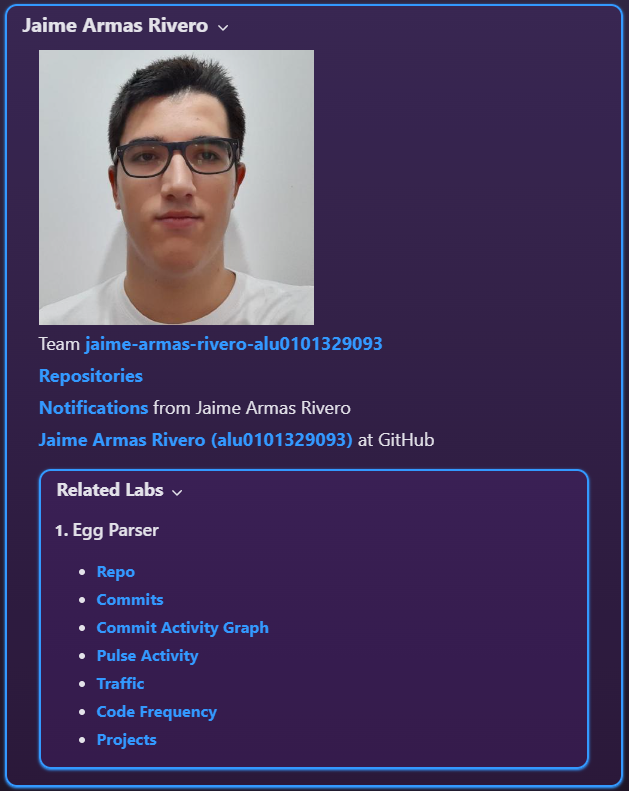
\includegraphics{images/userInfoCard.png}
    \caption{Carta con la información de un estudiante}
    \label{fig:userInfoCard}
\end{figure}